% fig_summary_table.tex — TR-12 HIF sensitivity comparison table (TikZ)
% Columns: Zone | Method | α50 before | α50 after | I_f,50 before | I_f,50 after | Delta
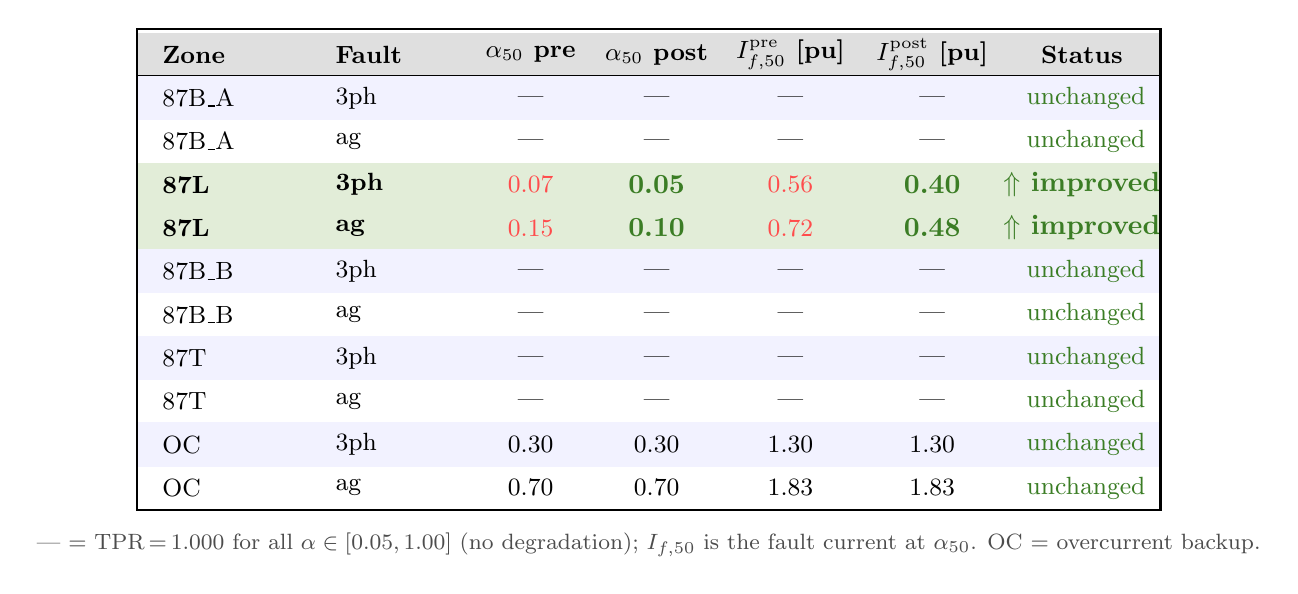
\begin{tikzpicture}[font=\small]

% Column x positions
\def\cA{0.0}  % Zone
\def\cB{2.2}  % Method
\def\cC{4.2}  % alpha50 before
\def\cD{5.8}  % alpha50 after
\def\cE{7.4}  % I_f,50 before [pu]
\def\cF{9.2}  % I_f,50 after [pu]
\def\cG{11.0} % Improved?

\def\rowH{0.55}  % row height

% Header background
\fill[gray!25] (-.2,0.05) rectangle (12.8,\rowH+0.05);

% Header row
\node[anchor=west,font=\small\bfseries] at (\cA, 0.32) {Zone};
\node[anchor=west,font=\small\bfseries] at (\cB, 0.32) {Fault};
\node[anchor=center,font=\small\bfseries] at (\cC+0.6, 0.32) {$\alpha_{50}$ pre};
\node[anchor=center,font=\small\bfseries] at (\cD+0.6, 0.32) {$\alpha_{50}$ post};
\node[anchor=center,font=\small\bfseries] at (\cE+0.7, 0.32) {$I_{f,50}^{\rm pre}$ [pu]};
\node[anchor=center,font=\small\bfseries] at (\cF+0.7, 0.32) {$I_{f,50}^{\rm post}$ [pu]};
\node[anchor=center,font=\small\bfseries] at (\cG+0.8, 0.32) {Status};

% Separator below header
\draw[thick] (-.2,0.05) -- (12.8,0.05);

% Data rows  (y starts at -rowH/2, decrements by rowH)
% Row 1: 87B_A 3ph
\def\ry{-0.23}
\fill[blue!5] (-.2,\ry-0.28) rectangle (12.8,\ry+0.28);
\node[anchor=west] at (\cA,\ry) {87B\_A};
\node[anchor=west] at (\cB,\ry) {3ph};
\node[anchor=center] at (\cC+0.6,\ry) {---};
\node[anchor=center] at (\cD+0.6,\ry) {---};
\node[anchor=center] at (\cE+0.7,\ry) {---};
\node[anchor=center] at (\cF+0.7,\ry) {---};
\node[anchor=center,text=OliveGreen] at (\cG+0.8,\ry) {$\checkmark$ unchanged};

% Row 2: 87B_A ag
\def\ry{-0.78}
\node[anchor=west] at (\cA,\ry) {87B\_A};
\node[anchor=west] at (\cB,\ry) {ag};
\node[anchor=center] at (\cC+0.6,\ry) {---};
\node[anchor=center] at (\cD+0.6,\ry) {---};
\node[anchor=center] at (\cE+0.7,\ry) {---};
\node[anchor=center] at (\cF+0.7,\ry) {---};
\node[anchor=center,text=OliveGreen] at (\cG+0.8,\ry) {$\checkmark$ unchanged};

% Row 3: 87L 3ph — key row
\def\ry{-1.33}
\fill[OliveGreen!12] (-.2,\ry-0.28) rectangle (12.8,\ry+0.28);
\node[anchor=west,font=\small\bfseries] at (\cA,\ry) {87L};
\node[anchor=west,font=\small\bfseries] at (\cB,\ry) {3ph};
\node[anchor=center,text=red!70] at (\cC+0.6,\ry) {0.07};
\node[anchor=center,text=OliveGreen,font=\bfseries] at (\cD+0.6,\ry) {0.05};
\node[anchor=center,text=red!70] at (\cE+0.7,\ry) {0.56};
\node[anchor=center,text=OliveGreen,font=\bfseries] at (\cF+0.7,\ry) {0.40};
\node[anchor=center,text=OliveGreen,font=\bfseries] at (\cG+0.8,\ry) {$\Uparrow$ improved};

% Row 4: 87L ag — key row
\def\ry{-1.88}
\fill[OliveGreen!12] (-.2,\ry-0.28) rectangle (12.8,\ry+0.28);
\node[anchor=west,font=\small\bfseries] at (\cA,\ry) {87L};
\node[anchor=west,font=\small\bfseries] at (\cB,\ry) {ag};
\node[anchor=center,text=red!70] at (\cC+0.6,\ry) {0.15};
\node[anchor=center,text=OliveGreen,font=\bfseries] at (\cD+0.6,\ry) {0.10};
\node[anchor=center,text=red!70] at (\cE+0.7,\ry) {0.72};
\node[anchor=center,text=OliveGreen,font=\bfseries] at (\cF+0.7,\ry) {0.48};
\node[anchor=center,text=OliveGreen,font=\bfseries] at (\cG+0.8,\ry) {$\Uparrow$ improved};

% Row 5: 87B_B 3ph
\def\ry{-2.43}
\fill[blue!5] (-.2,\ry-0.28) rectangle (12.8,\ry+0.28);
\node[anchor=west] at (\cA,\ry) {87B\_B};
\node[anchor=west] at (\cB,\ry) {3ph};
\node[anchor=center] at (\cC+0.6,\ry) {---};
\node[anchor=center] at (\cD+0.6,\ry) {---};
\node[anchor=center] at (\cE+0.7,\ry) {---};
\node[anchor=center] at (\cF+0.7,\ry) {---};
\node[anchor=center,text=OliveGreen] at (\cG+0.8,\ry) {$\checkmark$ unchanged};

% Row 6: 87B_B ag
\def\ry{-2.98}
\node[anchor=west] at (\cA,\ry) {87B\_B};
\node[anchor=west] at (\cB,\ry) {ag};
\node[anchor=center] at (\cC+0.6,\ry) {---};
\node[anchor=center] at (\cD+0.6,\ry) {---};
\node[anchor=center] at (\cE+0.7,\ry) {---};
\node[anchor=center] at (\cF+0.7,\ry) {---};
\node[anchor=center,text=OliveGreen] at (\cG+0.8,\ry) {$\checkmark$ unchanged};

% Row 7: 87T 3ph
\def\ry{-3.53}
\fill[blue!5] (-.2,\ry-0.28) rectangle (12.8,\ry+0.28);
\node[anchor=west] at (\cA,\ry) {87T};
\node[anchor=west] at (\cB,\ry) {3ph};
\node[anchor=center] at (\cC+0.6,\ry) {---};
\node[anchor=center] at (\cD+0.6,\ry) {---};
\node[anchor=center] at (\cE+0.7,\ry) {---};
\node[anchor=center] at (\cF+0.7,\ry) {---};
\node[anchor=center,text=OliveGreen] at (\cG+0.8,\ry) {$\checkmark$ unchanged};

% Row 8: 87T ag
\def\ry{-4.08}
\node[anchor=west] at (\cA,\ry) {87T};
\node[anchor=west] at (\cB,\ry) {ag};
\node[anchor=center] at (\cC+0.6,\ry) {---};
\node[anchor=center] at (\cD+0.6,\ry) {---};
\node[anchor=center] at (\cE+0.7,\ry) {---};
\node[anchor=center] at (\cF+0.7,\ry) {---};
\node[anchor=center,text=OliveGreen] at (\cG+0.8,\ry) {$\checkmark$ unchanged};

% Row 9: OC 3ph
\def\ry{-4.63}
\fill[blue!5] (-.2,\ry-0.28) rectangle (12.8,\ry+0.28);
\node[anchor=west] at (\cA,\ry) {OC};
\node[anchor=west] at (\cB,\ry) {3ph};
\node[anchor=center] at (\cC+0.6,\ry) {0.30};
\node[anchor=center] at (\cD+0.6,\ry) {0.30};
\node[anchor=center] at (\cE+0.7,\ry) {1.30};
\node[anchor=center] at (\cF+0.7,\ry) {1.30};
\node[anchor=center,text=OliveGreen] at (\cG+0.8,\ry) {$\checkmark$ unchanged};

% Row 10: OC ag
\def\ry{-5.18}
\node[anchor=west] at (\cA,\ry) {OC};
\node[anchor=west] at (\cB,\ry) {ag};
\node[anchor=center] at (\cC+0.6,\ry) {0.70};
\node[anchor=center] at (\cD+0.6,\ry) {0.70};
\node[anchor=center] at (\cE+0.7,\ry) {1.83};
\node[anchor=center] at (\cF+0.7,\ry) {1.83};
\node[anchor=center,text=OliveGreen] at (\cG+0.8,\ry) {$\checkmark$ unchanged};

% Bottom line
\draw[thick] (-.2,-5.46) -- (12.8,-5.46);
% Top line
\draw[thick] (-.2,0.65) -- (12.8,0.65);
% Outer border
\draw[thick] (-.2,0.65) rectangle (12.8,-5.46);

% Note below
\node[font=\footnotesize,align=left,text=gray!60!black] at (6.3,-5.9)
  {--- = TPR\,=\,1.000 for all $\alpha \in [0.05,1.00]$ (no degradation);
   $I_{f,50}$ is the fault current at $\alpha_{50}$. OC = overcurrent backup.};

\end{tikzpicture}
